\documentclass{ximera}

\input{../preamble.tex}

\outcome{Understand the properties of trigonometric functions.}
\outcome{Evaluate expressions and solve equations involving
          trigonometric functions and inverse trigonometric functions.}
\outcome{Evaluate limits involving trigonometric functions.}

\title[Dig-In:]{Trigonometric functions}

\begin{document}
\begin{abstract}
  We review trigonometric functions.
\end{abstract}
\maketitle



\section{What are trigonometric functions?}

\begin{definition}
  A \dfn{trigonometric function} is a function that relates a measure
  of an angle of a right triangle to a ratio of the triangle's sides.
\end{definition}


The basic trigonometric functions are cosine and sine. They are called
``trigonometric'' because they relate measures of angles to
measurements of triangles. Given a right triangle
\begin{image}[2in]
  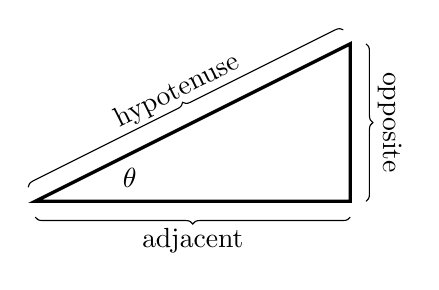
\begin{tikzpicture}
    \coordinate (C) at (0,2);
    \coordinate (D) at (4,2);
    \coordinate (E) at (4,4);
    \tkzMarkRightAngle(C,D,E)
    \tkzMarkAngle(D,C,E)
    \draw[decoration={brace,mirror,raise=.2cm},decorate,thin] (0,2)--(4,2);
    \draw[decoration={brace,mirror,raise=.2cm},decorate,thin] (4,2)--(4,4);
    \draw[decoration={brace,raise=.2cm},decorate,thin] (0,2)--(4,4);
    \draw[very thick] (D)--(E)--(C)--cycle;
    \node at (2,2-.5) {adjacent};
    \node[rotate=-90] at (4+.5,3) {opposite};
    \node[rotate=26.5] at (2-.2,3+.4) {hypotenuse};
    \node at (1.2,2.3) {$\theta$};
  \end{tikzpicture}
\end{image}
we define
\[
\cos(\theta) =
\frac{\text{adjacent}}{\text{hypotenuse}}\qquad\text{and}\qquad\sin(\theta)
= \frac{\text{opposite}}{\text{hypotenuse}}.
\]
Note, the values of sine and cosine do not depend on the scale of the
triangle. Being very explicit, if we scale a triangle by a scale
factor $k$,

\begin{image}[2in]
      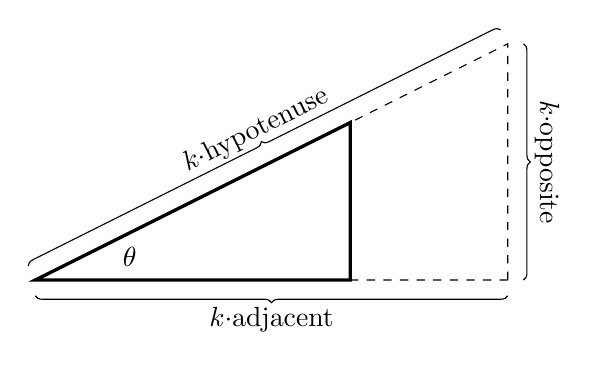
\begin{tikzpicture}
      \coordinate (A) at (6,2);
      \coordinate (B) at (6,5);
      \coordinate (C) at (0,2);
      \coordinate (D) at (4,2);
      \coordinate (E) at (4,4);
      \tkzMarkRightAngle(C,A,B)
      \tkzMarkRightAngle(C,D,E)
      \tkzMarkAngle(D,C,E)
      
      
      \draw[decoration={brace,mirror,raise=.2cm},decorate,thin] (0,2)--(6,2);
      \draw[decoration={brace,mirror,raise=.2cm},decorate,thin] (6,2)--(6,5);
      \draw[decoration={brace,raise=.2cm},decorate,thin] (0,2)--(6,5);
      \draw[dashed] (A)--(B)--(C)--cycle;
      \draw[very thick] (D)--(E)--(C)--cycle;
      \node at (3,2-.5) {\text{$k\cdot$adjacent}};
      \node[rotate=-90] at (6+.5,3.5) {$k\cdot$opposite};
      \node[rotate=26.5] at (3-.2,3.5+.4) {$k\cdot$hypotenuse};
      \node at (1.2,2.3) {$\theta$};
      \end{tikzpicture}
\end{image}
\[
\cos(\theta) = \frac{k\cdot\text{adjacent}}{k\cdot\text{hypotenuse}} =\frac{\text{adjacent}}{\text{hypotenuse}}
\]
and
\[
\sin(\theta) = \frac{k\cdot\text{opposite}}{k\cdot\text{hypotenuse}} = \frac{\text{opposite}}{\text{hypotenuse}}.
\]

At this point we could simply assume that whenever we draw a triangle
for computing sine and cosine, that the hypotenuse will be $1$. We can
do this because we are simply scaling the triangle, and as we see
above, this makes absolutely no difference when computing sine and
cosine. Hence, when the hypotenuse is $1$, we find that a convenient
way to think about sine and cosine is via the unit circle:
\begin{image}
\begin{tikzpicture}
	\begin{axis}[
            xmin=-1.1,xmax=1.1,ymin=-1.1,ymax=1.1,
            axis lines=center,
            width=4in,
            xtick={-1,1},
            ytick={-1,1},
            clip=false,
            unit vector ratio*=1 1 1,
            xlabel=$x$, ylabel=$y$,
            every axis y label/.style={at=(current axis.above origin),anchor=south},
            every axis x label/.style={at=(current axis.right of origin),anchor=west},
          ]        
          \addplot [dashed, smooth, domain=(0:360)] ({cos(x)},{sin(x)}); %% unit circle

          \addplot [textColor] plot coordinates {(0,0) (.766,.643)}; %% 40 degrees

          \addplot [ultra thick,penColor] plot coordinates {(.766,0) (.766,.643)}; %% 40 degrees
          \addplot [ultra thick,penColor2] plot coordinates {(0,0) (.766,0)}; %% 40 degrees
          
          %\addplot [ultra thick,penColor3] plot coordinates {(1,0) (1,.839)}; %% 40 degrees          

          \addplot [textColor,smooth, domain=(0:40)] ({.15*cos(x)},{.15*sin(x)});
          %\addplot [very thick,penColor] plot coordinates {(0,0) (.766,.643)}; %% sector
          %\addplot [very thick,penColor] plot coordinates {(0,0) (1,0)}; %% sector
          %\addplot [very thick, penColor, smooth, domain=(0:40)] ({cos(x)},{sin(x)}); %% sector
          \node at (axis cs:.15,.07) [anchor=west] {$\theta$};
          \node[penColor, rotate=-90] at (axis cs:.84,.322) {$\sin(\theta)$};
          \node[penColor2] at (axis cs:.383,0) [anchor=north] {$\cos(\theta)$};
          %\node[penColor3, rotate=-90] at (axis cs:1.06,.322) {$\tan(\theta)$};
        \end{axis}
\end{tikzpicture}
\end{image}

If we consider all possible combinations of ratios of
\begin{center}
  adjacent, \qquad opposite, \qquad hypotenuse,
\end{center}
(allowing the adjacent and opposite to be negative, as on the unit
circle) we obtain all of the trigonometric functions.

\begin{definition}
  \index{sine}
  \index{cosine}
  \index{tangent}
  \index{secant}
  \index{cosecant}
  \index{cotangent}
  The trigonometric functions\index{trigonometric function} are:
  \[
  \begin{aligned}
  \cos(\theta) &= \frac{\text{adj}}{\text{hyp}}\\
  \sec(\theta) &= \frac{1}{\cos(\theta)}\\
  \tan(\theta) &= \frac{\sin(\theta)}{\cos(\theta)}\qquad
  \end{aligned}
  \qquad
  \begin{aligned}
  \sin(\theta) &= \frac{\text{opp}}{\text{hyp}}\\
  \csc(\theta) &= \frac{1}{\sin(\theta)}\\
  \cot(\theta) &= \frac{\cos(\theta)}{\sin(\theta)}    
  \end{aligned}
  \]
  where the domain of sine and cosine is all real numbers, and the
  other trigonometric functions are defined precisely when their
  denominators are nonzero.
\end{definition}

\begin{question}
  Which of the following expressions are equal to $\sec(\theta)$?
  \begin{selectAll}
    \choice[correct]{$\frac{1}{\cos(\theta)}$}
    \choice{$\frac{1}{\sin(\theta)}$}
    \choice{$\frac{\text{adj}}{\text{hyp}}$}
    \choice[correct]{$\frac{\text{hyp}}{\text{adj}}$}
    \choice{$\frac{\tan(\theta)}{\sin(\theta)}$}
    \choice{$\frac{1}{\sin(\theta)\cdot\cot(\theta)}$}
  \end{selectAll}
  \begin{feedback}
    Note, $\frac{\tan(\theta)}{\sin(\theta)}\ne \sec(\theta)$, and
    $\frac{1}{\sin(\theta)\cdot\cot(\theta)}\ne \sec(\theta)$ since
    they differ when $\theta =0$.
  \end{feedback}
\end{question}


\section{Not all angles come from triangles.}
Given a right triangle like
\begin{image}[2in]
  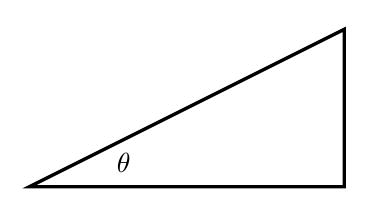
\begin{tikzpicture}
    \coordinate (C) at (0,2);
    \coordinate (D) at (4,2);
    \coordinate (E) at (4,4);
    \tkzMarkRightAngle(C,D,E)
    \tkzMarkAngle(D,C,E)
    \draw[very thick] (D)--(E)--(C)--cycle;
    \node at (1.2,2.3) {$\theta$};
  \end{tikzpicture}
\end{image}
the angle $\theta$ cannot exceed $\frac{\pi}{2}$ radians.  That means to talk about trigonometric functions for \emph{other} angles, we need to be able
to describe the trigonometric functions a little more generally.  To do this, we use the unit circle from the previous section.  Given an angle $\theta$,
we construct the angle with initial side along the positive $x$-axis and vertex at the origin.

\begin{image}
\begin{tikzpicture}
	\begin{axis}[
            xmin=-1.1,xmax=1.1,ymin=-1.1,ymax=1.1,
            axis lines=center,
            width=4in,
            xtick={-1,1},
            ytick={-1,1},
            clip=false,
            unit vector ratio*=1 1 1,
            xlabel=$x$, ylabel=$y$,
            every axis y label/.style={at=(current axis.above origin),anchor=south},
            every axis x label/.style={at=(current axis.right of origin),anchor=west},
          ]        
          \addplot [dashed, smooth, domain=(0:360)] ({cos(x)},{sin(x)}); %% unit circle
          \addplot [thick, penColor] plot coordinates {(0,0) (.766,.643)}; %% 40 degrees
          \addplot [thick, penColor2] plotcoordinates {(0,0) (1,0)};
          \addplot [textColor,smooth, domain=(0:40)] ({.15*cos(x)},{.15*sin(x)});
          \node at (axis cs:.15,.07) [anchor=west] {$\theta$};
          \node[textColor, rotate=40] at (axis cs:.35,.38) {terminal side};
          \node[textColor] at (axis cs:.5,-.07) {initial side};
%          \draw (.766, .643) node[circle,fill,inner sep=1pt, label=above:$(\cos \theta, \sin \theta)$](a){};
        \end{axis}
\end{tikzpicture}
\end{image}
As the angle $\theta$ grows larger and larger, the terminal side of that angle spins around the circle.
The trigonometric functions of the angle $\theta$ are defined in terms of the terminal side.  
\begin{definition}
	Suppose $(x,y)$ is the point at which the terminal side of the angle with measure $\theta$ intersects the unit circle.
	The the trigonometric functions are defined to be
	\[\begin{aligned}
  		\cos(\theta) &= x\\
  		\sec(\theta) &= \frac{1}{x}\\
  		\tan(\theta) &= \frac{y}{x}\qquad
  	\end{aligned}
  	\qquad
  	\begin{aligned}
  		\sin(\theta) &= y\\
  		\csc(\theta) &= \frac{1}{y}\\
  		\cot(\theta) &= \frac{x}{y}    
	\end{aligned}\]
	provided these values exist.
\end{definition}
From the picture, you see that this agrees with what you know about trigonometry for triangles, but it allows us to extend the definition of sine and cosine to
all real numbers, instead of only the interval $\left( 0, \frac{\pi}{2} \right)$



\section{Graphs}
As a reminder, we include the graphs here.

\begin{image}
\begin{tikzpicture}
	\begin{axis}[
            xmin=-6.75,xmax=6.75,ymin=-1.5,ymax=1.5,
            axis lines=center,
            xtick={-6.28, -4.71, -3.14, -1.57, 0, 1.57, 3.142, 4.71, 6.28},
            xticklabels={$-2\pi$,$-3\pi/2$,$-\pi$, $-\pi/2$, $0$, $\pi/2$, $\pi$, $3\pi/2$, $2\pi$},
            ytick={-1,1},
            %ticks=none,
            width=6in,
            height=3in,
            unit vector ratio*=1 1 1,
            xlabel=$\theta$, ylabel=$x$,
            every axis y label/.style={at=(current axis.above origin),anchor=south},
            every axis x label/.style={at=(current axis.right of origin),anchor=west},
          ]        
          \addplot [very thick, penColor, samples=300,smooth, domain=(-6.75:6.75)] {sin(deg(x))};
          \node at (axis cs:-1.57,.75) [penColor2] {$\sin(\theta)$};
        \end{axis}
\end{tikzpicture}
\end{image}

\begin{image}
\begin{tikzpicture}
	\begin{axis}[
            xmin=-6.75,xmax=6.75,ymin=-1.5,ymax=1.5,
            axis lines=center,
            xtick={-6.28, -4.71, -3.14, -1.57, 0, 1.57, 3.142, 4.71, 6.28},
            xticklabels={$-2\pi$,$-3\pi/2$,$-\pi$, $-\pi/2$, $0$, $\pi/2$, $\pi$, $3\pi/2$, $2\pi$},
            ytick={-1,1},
            %ticks=none,
            width=6in,
            height=3in,
            unit vector ratio*=1 1 1,
            xlabel=$\theta$, ylabel=$x$,
            every axis y label/.style={at=(current axis.above origin),anchor=south},
            every axis x label/.style={at=(current axis.right of origin),anchor=west},
          ]        
          \addplot [very thick, penColor, samples=300,smooth, domain=(-6.75:6.75)] {cos(deg(x))};
          \node at (axis cs:-1.57,.75) [penColor2] {$\cos(\theta)$};
        \end{axis}
\end{tikzpicture}
\end{image}


\begin{image}
\begin{tikzpicture}
	\begin{axis}[
            xmin=-6.75,xmax=6.75,ymin=-5.5,ymax=5.5,
            axis lines=center,
            xtick={-6.28, -4.71, -3.14, -1.57, 0, 1.57, 3.142, 4.71, 6.28},
            xticklabels={$-2\pi$,$-3\pi/2$,$-\pi$, $-\pi/2$, $0$, $\pi/2$, $\pi$, $3\pi/2$, $2\pi$},
            ytick={-1,1},
            %ticks=none,
            width=6in,
            height=3in,
            unit vector ratio*=1 1 1,
            xlabel=$\theta$, ylabel=$x$,
            every axis y label/.style={at=(current axis.above origin),anchor=south},
            every axis x label/.style={at=(current axis.right of origin),anchor=west},
          ]        
          \addplot [very thick, penColor, samples=100,smooth, domain=(-1.56:1.56)] {tan(deg(x))};
          \addplot [very thick, penColor, samples=100,smooth, domain=(1.58:4.7)] {tan(deg(x))};
          \addplot [very thick, penColor, samples=100,smooth, domain=(4.9:6.28)] {tan(deg(x))};
          \addplot [very thick, penColor, samples=100,smooth, domain=(-4.7:-1.58)] {tan(deg(x))};
          \addplot [very thick, penColor, samples=100,smooth, domain=(-6.28:-4.9)] {tan(deg(x))};          
          \node at (axis cs:-0.7,2) [penColor2] {$\tan(\theta)$};
        \end{axis}
\end{tikzpicture}
\end{image}

\begin{image}
\begin{tikzpicture}
	\begin{axis}[
            xmin=-6.75,xmax=6.75,ymin=-5.5,ymax=5.5,
            axis lines=center,
            xtick={-6.28, -4.71, -3.14, -1.57, 0, 1.57, 3.142, 4.71, 6.28},
            xticklabels={$-2\pi$,$-3\pi/2$,$-\pi$, $-\pi/2$, $0$, $\pi/2$, $\pi$, $3\pi/2$, $2\pi$},
            ytick={-1,1},
            %ticks=none,
            width=6in,
            height=3in,
            unit vector ratio*=1 1 1,
            xlabel=$\theta$, ylabel=$x$,
            every axis y label/.style={at=(current axis.above origin),anchor=south},
            every axis x label/.style={at=(current axis.right of origin),anchor=west},
          ]        
          \addplot [very thick, penColor, samples=100,smooth, domain=(3.15:6.27)] {cot(deg(x))};
          \addplot [very thick, penColor, samples=100,smooth, domain=(0.01:3.13)] {cot(deg(x))};
          \addplot [very thick, penColor, samples=100,smooth, domain=(-3.13:-0.01)] {cot(deg(x))};
          \addplot [very thick, penColor, samples=100,smooth, domain=(-6.27:-3.15)] {cot(deg(x))};          
          \node at (axis cs:-0.7,2) [penColor2] {$\cot(\theta)$};
        \end{axis}
\end{tikzpicture}
\end{image}


\begin{image}
\begin{tikzpicture}
	\begin{axis}[
            xmin=-6.75,xmax=6.75,ymin=-5.5,ymax=5.5,
            axis lines=center,
            xtick={-6.28, -4.71, -3.14, -1.57, 0, 1.57, 3.142, 4.71, 6.28},
            xticklabels={$-2\pi$,$-3\pi/2$,$-\pi$, $-\pi/2$, $0$, $\pi/2$, $\pi$, $3\pi/2$, $2\pi$},
            ytick={-1,1},
            %ticks=none,
            width=6in,
            height=3in,
            unit vector ratio*=1 1 1,
            xlabel=$\theta$, ylabel=$x$,
            every axis y label/.style={at=(current axis.above origin),anchor=south},
            every axis x label/.style={at=(current axis.right of origin),anchor=west},
          ]        
          \addplot [very thick, penColor, samples=100,smooth, domain=(-1.56:1.56)] {sec(deg(x))};
          \addplot [very thick, penColor, samples=100,smooth, domain=(1.58:4.7)] {sec(deg(x))};
          \addplot [very thick, penColor, samples=100,smooth, domain=(4.9:6.28)] {sec(deg(x))};
          \addplot [very thick, penColor, samples=100,smooth, domain=(-4.7:-1.58)] {sec(deg(x))};
          \addplot [very thick, penColor, samples=100,smooth, domain=(-6.28:-4.9)] {sec(deg(x))};          
          \node at (axis cs:-2.0,0.5) [penColor2] {$\sec(\theta)$};
        \end{axis}
\end{tikzpicture}
\end{image}

\begin{image}
\begin{tikzpicture}
	\begin{axis}[
            xmin=-6.75,xmax=6.75,ymin=-5.5,ymax=5.5,
            axis lines=center,
            xtick={-6.28, -4.71, -3.14, -1.57, 0, 1.57, 3.142, 4.71, 6.28},
            xticklabels={$-2\pi$,$-3\pi/2$,$-\pi$, $-\pi/2$, $0$, $\pi/2$, $\pi$, $3\pi/2$, $2\pi$},
            ytick={-1,1},
            %ticks=none,
            width=6in,
            height=3in,
            unit vector ratio*=1 1 1,
            xlabel=$\theta$, ylabel=$x$,
            every axis y label/.style={at=(current axis.above origin),anchor=south},
            every axis x label/.style={at=(current axis.right of origin),anchor=west},
          ]        
          \addplot [very thick, penColor, samples=100,smooth, domain=(3.15:6.27)] {1/sin(deg(x))};
          \addplot [very thick, penColor, samples=100,smooth, domain=(0.01:3.13)] {1/sin(deg(x))};
          \addplot [very thick, penColor, samples=100,smooth, domain=(-3.13:-0.01)] {1/sin(deg(x))};
          \addplot [very thick, penColor, samples=100,smooth, domain=(-6.27:-3.15)] {1/sin(deg(x))};          
          \node at (axis cs:-1.2,2) [penColor2] {$\csc(\theta)$};
        \end{axis}
\end{tikzpicture}
\end{image}
%%%%
%%%  Finish this! 
%%%% 


\section{The power of the Pythagorean Theorem}

The Pythagorean Theorem is probably the most famous theorem in all of
mathematics.


\begin{theorem}[Pythagorean Theorem]\index{Pythagorean Theorem}
Given a right triangle:
\begin{image}[2in]
  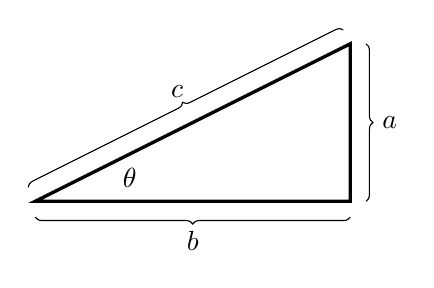
\begin{tikzpicture}
    \coordinate (C) at (0,2);
    \coordinate (D) at (4,2);
    \coordinate (E) at (4,4);
    \tkzMarkRightAngle(C,D,E)
    \tkzMarkAngle(D,C,E)
    \draw[decoration={brace,mirror,raise=.2cm},decorate,thin] (0,2)--(4,2);
    \draw[decoration={brace,mirror,raise=.2cm},decorate,thin] (4,2)--(4,4);
    \draw[decoration={brace,raise=.2cm},decorate,thin] (0,2)--(4,4);
    \draw[very thick] (D)--(E)--(C)--cycle;
    \node at (2,2-.5) {$b$};
    \node[] at (4+.5,3) {$a$};
    \node at (2-.2,3+.4) {$c$};
    \node at (1.2,2.3) {$\theta$};
  \end{tikzpicture}
\end{image}
We have that:
\[
a^2 + b^2 = c^2
\]
\end{theorem}


The Pythagorean Theorem gives several key trigonometric identities.

\begin{theorem}[Pythagorean Identities]\index{Pythagorean identities}
  The following hold:
  \[
  \cos^2\theta+\sin^2\theta = 1 \qquad 1 + \tan^2\theta = \sec^2\theta \qquad \cot^2\theta + 1 = \csc^2\theta
  \]
  \begin{explanation}
    From the unit circle we can see
    \begin{image}
\begin{tikzpicture}
	\begin{axis}[
            xmin=-1.1,xmax=1.1,ymin=-1.1,ymax=1.1,
            axis lines=center,
            width=4in,
            ticks=none,
            clip=false,
            unit vector ratio*=1 1 1,
            %xlabel=$x$, ylabel=$y$,
            every axis y label/.style={at=(current axis.above origin),anchor=south},
            every axis x label/.style={at=(current axis.right of origin),anchor=west},
          ]        
          \addplot [dashed, smooth, domain=(0:360)] ({cos(x)},{sin(x)}); %% unit circle

          \addplot [textColor] plot coordinates {(0,0) (.766,.643)}; %% 40 degrees

          \addplot [ultra thick,penColor] plot coordinates {(.766,0) (.766,.643)}; %% 40 degrees
          \addplot [ultra thick,penColor2] plot coordinates {(0,0) (.766,0)}; %% 40 degrees
          
          %\addplot [ultra thick,penColor3] plot coordinates {(1,0) (1,.839)}; %% 40 degrees          

          \addplot [textColor,smooth, domain=(0:40)] ({.15*cos(x)},{.15*sin(x)});
          %\addplot [very thick,penColor] plot coordinates {(0,0) (.766,.643)}; %% sector
          %\addplot [very thick,penColor] plot coordinates {(0,0) (1,0)}; %% sector
          %\addplot [very thick, penColor, smooth, domain=(0:40)] ({cos(x)},{sin(x)}); %% sector
          \node at (axis cs:.15,.07) [anchor=west] {$t$};
          \node[penColor, rotate=-90] at (axis cs:.84,.322) {$\sin(t)$};
          \node[penColor2] at (axis cs:.383,0) [anchor=north] {$\cos(t)$};
          %\node[penColor3, rotate=-90] at (axis cs:1.06,.322) {$\tan(\theta)$};
        \end{axis}
\end{tikzpicture}
    \end{image}
    via the Pythagorean Theorem that
    \[
    \cos^2(t) + \sin^2(t) = 1.
    \]
    If we divide this expression by $\answer[given]{\cos^2(t)}$ we obtain
    \[
    1 + \tan^2(t) = \sec^2(t)
    \]
    and if we divide $\cos^2(t) + \sin^2(t) = 1$ by $\answer[given]{\sin^2(t)}$ we obtain
    \[
    \cot^2(t) + 1 = \csc^2(t).
    \]
  \end{explanation}
\end{theorem}

%%%%%
%%   Add more trig identities to remember!  Angle addition, Double Angle, Half-Angleformulas.
%%%%%


\section{Trigonometric equations}
Frequently we are in the situation of having to determine precisely which angles satisfy a particular equation.  The most basic example is probably like this one.
\begin{example}
	Solve the equation: \[ \sin \theta = -\frac{1}{2}. \]
	\begin{explanation}
		We'll start by finding the reference angle.
	\end{explanation}
\end{example}

%%%%%%
%% More trig equations
%%%%%%




\section{Limits involving trigonometric functions}
Back when we introduced continuity we mentioned that each trigonometric function is continuous on its domain.

\begin{example}
	Compute the limit: \[ \lim_{\theta \to 2\pi/3} \theta \tan \theta. \]
	\begin{explanation}
		The multiplicative limit law allows us to split this into \[ \left(\lim_{\theta\to 2\pi/3} \theta \right) \left(\lim_{\theta\to 2\pi/3} \tan \theta \right). \]
		The function $f(\theta) = \theta$ is continuous everywhere, so $\lim_{\theta\to 2\pi/3} \theta = \answer[given]{\frac{2\pi}{3}}$.  Since $\frac{2 \pi}{3}$ is in the domain
		of $\tan \theta$, we have $\lim_{\theta\to 2\pi/3} \tan \theta = \tan \left( \answer[given]{\frac{2 \pi}{3}} \right) = - \sqrt{3}$.  Putting these together we find
		\[ \lim_{\theta\to 2\pi/3} \theta \tan \theta = - \frac{2 \pi \sqrt{3}}{3}. \]
	\end{explanation}
\end{example}


\begin{example}
	Compute the limit: \[ \lim_{\theta \to \pi^-} \cot \theta. \]
	\begin{explanation}
		Recall that $\cot \theta = \frac{\cos \theta}{\sin \theta}$, so that \[ \lim_{\theta \to \pi^-} \cot \theta = \lim_{\theta \to \pi^-} \frac{\cos \theta}{\sin \theta}.\]
		Since sine and cosine are continuous, $\lim_{\theta \to \pi^-} \cos \theta = \cos\left( \answer[given]{\pi} \right)= \answer[given]{-1}$ and 
		$\lim_{\theta \to \pi^-} \sin \theta = \sin\left( \answer[given]{\pi} \right)  = \answer[given]{0}$.
		That is, $\lim_{\theta \to \pi^-} \cot \theta$ is of the form $\numOverZero$.
		
		The numerator is negative for $\theta$ near $\pi$.  From the graph of $\sin \theta$, we know that the denominator is negative and approaching $0$ as $\theta \to \pi^{-}$.
		That means \[ \lim_{\theta \to \pi^-} \cot \theta = -\infty. \]
	\end{explanation}
\end{example}



\begin{question}
	Compute the limit: 
	\[ \lim_{\theta \to \frac{\pi}{12} } \frac{ 2\cos\left( 4 \theta \right) \sin\left( 6 \theta \right) }{ \theta } = \answer{ \frac{12}{\pi} } \]
\end{question}



We'll end with a couple very involved limits where the Squeeze Theorem makes a surprising return.

\begin{example}
Compute:
\[
\lim_{\theta\to 0} \frac{\sin(\theta)}{\theta}
\]
\begin{explanation}
To compute this limit, use the Squeeze Theorem. First note that we
only need to examine $\theta\in \left(\frac{-\pi}{2}, \frac{\pi}{2}\right)$
and for the present time, we'll assume that $\theta$ is positive. Consider
the diagrams below:

\begin{image}
\begin{tabular}{ccc}
\begin{tikzpicture}
	\begin{axis}[
            xmin=-.1,xmax=1.1,ymin=-.1,ymax=1.1,
            axis lines=center,
            ticks=none,
            clip=false,
            unit vector ratio*=1 1 1,
            xlabel=$x$, ylabel=$y$,
            every axis y label/.style={at=(current axis.above origin),anchor=south},
            every axis x label/.style={at=(current axis.right of origin),anchor=west},
          ]        
          \addplot [very thick, penColor2, smooth, domain=(-.1:.2+pi/2)] ({cos(deg(x))},{sin(deg(x))});
          \addplot [textColor] plot coordinates {(0,0) (1,.839)}; %% 40 degrees
          \addplot [very thick, penColor] plot coordinates {(.766,0) (.766,.643)}; %% 40 degrees
          \addplot [textColor] plot coordinates {(1,0) (1,.839)}; %% 40 degrees
          \addplot [very thick,penColor,fill=fill1] plot coordinates {(0,0) (.766,.643)}\closedcycle; %% triangle
          \addplot [textColor,smooth, domain=(0:40)] ({.15*cos(x)},{.15*sin(x)});
          \node at (axis cs:.15,.07) [anchor=west] {$\theta$};
          \node at (axis cs:.766,.322) [anchor=east] {$\sin(\theta)$};
          \node at (axis cs:.383,0) [anchor=north] {$\cos(\theta)$};
          \node at (axis cs:.5,-.1) [anchor=north] {Triangle $A$};
        \end{axis}
\end{tikzpicture} & 
\begin{tikzpicture}
  \begin{axis}[
      clip=false,
      xmin=-.1,xmax=1.1,ymin=-.1,ymax=1.1,
      axis lines=center,
      ticks=none,
      unit vector ratio*=1 1 1,
      xlabel=$x$, ylabel=$y$,
      every axis y label/.style={at=(current axis.above origin),anchor=south},
      every axis x label/.style={at=(current axis.right of origin),anchor=west},
    ]        
    \addplot [draw=none,fill=fill1] plot coordinates {(0,0) (.766,.643)}\closedcycle; %% sector
    \addplot [draw=none, fill=fill1, samples=100, domain=(0:40)] ({cos(x)},{sin(x)})\closedcycle; %% sector 
    \addplot [very thick, penColor2, smooth, domain=(-.1:.2+pi/2)] ({cos(deg(x))},{sin(deg(x))});
    \addplot [textColor] plot coordinates {(0,0) (1,.839)}; %% 40 degrees
    \addplot [textColor] plot coordinates {(.766,0) (.766,.643)}; %% 40 degrees
    \addplot [textColor] plot coordinates {(1,0) (1,.839)}; %% 40 degrees          
    \addplot [textColor,smooth, domain=(0:40)] ({.15*cos(x)},{.15*sin(x)});
    \addplot [very thick,penColor] plot coordinates {(0,0) (.766,.643)}; %% sector
    \addplot [very thick,penColor] plot coordinates {(0,0) (1,0)}; %% sector
    \addplot [very thick, penColor, smooth, domain=(0:40)] ({cos(x)},{sin(x)}); %% sector
    \node at (axis cs:.15,.07) [anchor=west] {$\theta$};
    \node at (axis cs:.5,0) [anchor=north] {$1$};
    \node at (axis cs:.5,-.1) [anchor=north] {Sector};
  \end{axis}
\end{tikzpicture} & 
\begin{tikzpicture}
  \begin{axis}[
      clip=false,
      xmin=-.1,xmax=1.1,ymin=-.1,ymax=1.1,
      axis lines=center,
      ticks=none,
      unit vector ratio*=1 1 1,
      xlabel=$x$, ylabel=$y$,
      every axis y label/.style={at=(current axis.above origin),anchor=south},
      every axis x label/.style={at=(current axis.right of origin),anchor=west},
    ]        
    \addplot [very thick,penColor,fill=fill1] plot coordinates {(0,0) (1,.839)}\closedcycle; %% triangle          
    \addplot [very thick, penColor2, smooth, domain=(-.1:1.671)] ({cos(deg(x))},{sin(deg(x))});
    \addplot [very thick, penColor] plot coordinates {(0,0) (1,.839)}; %% 40 degrees
    \addplot [textColor] plot coordinates {(.766,0) (.766,.643)}; %% 40 degrees
    \addplot [very thick, penColor] plot coordinates {(1,0) (1,.839)}; %% 40 degrees          
    \addplot [textColor,smooth, domain=(0:40)] ({.15*cos(x)},{.15*sin(x)});
    \node at (axis cs:.15,.07) [anchor=west] {$\theta$};
    \node at (axis cs:.5,0) [anchor=north] {$1$};
    \node at (axis cs:1,.42) [anchor=west] {$\tan(\theta)$};
    \node at (axis cs:.5,-.1) [anchor=north] {Triangle $B$};
  \end{axis}
\end{tikzpicture}
\end{tabular}
\end{image}


From our diagrams above we see that
\[
\text{Area of Triangle $A$} \le \text{Area of Sector} \le \text{Area of Triangle $B$}
\]
and computing these areas we find
\[
\frac{\cos(\theta)\sin(\theta)}{2} \le \frac{\theta}{2} \le \frac{\tan(\theta)}{2}.
\]
Multiplying through by $2$, and recalling that $\tan(\theta) =
\frac{\sin(\theta)}{\cos(\theta)}$ we obtain
\[
\cos(\theta)\sin(\theta) \le \theta \le \frac{\sin(\theta)}{\cos(\theta)}.
\]
Dividing through by $\sin(\theta)$ and taking the reciprocals
(reversing the inequalities), we find
\[
\cos(\theta) \le \frac{\sin(\theta)}{\theta} \le \frac{1}{\cos(\theta)}.
\]
Note, $\cos(-\theta) = \cos(\theta)$ and $\frac{\sin(-\theta)}{-\theta} =
\frac{\sin(\theta)}{\theta}$, so these inequalities hold for all $\theta\in
\left(\frac{-\pi}{2}, \frac{\pi}{2}\right)$.  Additionally, we know
\[
\lim_{\theta \to 0}\cos(\theta) = \answer[given]{1} = \lim_{\theta\to 0}\frac{1}{\cos(\theta)},
\]
and so we conclude by the Squeeze Theorem, $\lim_{\theta \to
  0}\frac{\sin(\theta)}{\theta} = \answer[given]{1}$.
\end{explanation}
\end{example}

When solving a problem with the Squeeze Theorem, one must write a sort
of mathematical poem. You have to tell your friendly reader exactly
which functions you are using to ``squeeze-out'' your limit.

\begin{example}
  Compute:
  \[
  \lim_{x\to 0} \left(\sin(x) e^{\cos\left(\frac{1}{x^3}\right)}\right)
  \]
  \begin{explanation}
    Let's graph this function to see what's going on:
    \begin{image}
      \begin{tikzpicture}
	\begin{axis}[
            domain=-4:4,    
            width=6in,
            height=3in,
            axis lines =middle, xlabel=$x$, ylabel=$y$,
            every axis y label/.style={at=(current axis.above origin),anchor=south},
            every axis x label/.style={at=(current axis.right of origin),anchor=west},
            clip=false,
            axis on top,
          ]
	  \addplot [very thick, penColor, smooth, samples=500,
            domain=(-4:-.35)] {sin(deg(x))*e^(cos(deg(1/x^3)))};
          \addplot [very thick, penColor, smooth, samples=500,
            domain=(.35:4)]  {sin(deg(x))*e^(cos(deg(1/x^3)))};
	  \addplot [color=penColor, fill=penColor,smooth,domain=(-.35:.35)] {sin(deg(x))*e} \closedcycle;
          \addplot [color=background, fill=background, smooth,domain=(-.35:.35)] {sin(deg(x)*1/e} \closedcycle;
          
          %\addplot [color=penColor, fill=penColor, very thick, smooth,domain=(-.3:0)] {-abs(sin(deg(x))*e)} \closedcycle;
          %\addplot [color=penColor, fill=penColor, very thick, smooth,domain=(-.3:0)] {abs(sin(deg(x)*1/e)} \closedcycle;
        \end{axis}
      \end{tikzpicture}
    \end{image}
    The function $\sin(x) e^{\cos\left(\frac{1}{x^3}\right)}$ has two factors:
    \begin{image}
      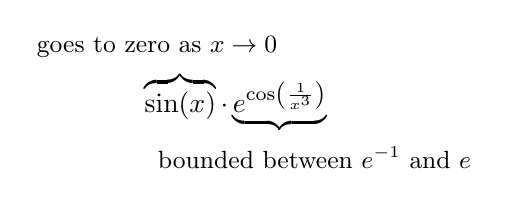
\begin{tikzpicture}
        \node at (0,0) {
          $\overbrace{\sin(x)} \cdot \underbrace{e^{\cos\left(\frac{1}{x^3}\right)}}$
          };
        \node at (-1,.7) {\small{goes to zero as $x\to 0$}};
        \node at (1,-.7) {\small{bounded between $e^{-1}$ and $e$}};
      \end{tikzpicture}
    \end{image}
    Hence we have that when $x>0$
    \[
    \sin(x) \answer[given]{e^{-1}} \le \sin(x) e^{\cos\left(\frac{1}{x^3}\right)} \le \sin(x) \answer[given]{e}
    \]
    and we see
    \[
    \lim_{x\to 0^+} \sin(x) \answer[given]{e^{-1}} = \answer[given]{0} = \lim_{x\to 0^+} \sin(x) \answer[given]{e}
    \]
    and so by the Squeeze theorem,
    \[
    \lim_{x\to
      0^+}\left(\sin(x)e^{\cos\left(\frac{1}{x^3}\right)}\right)=\answer[given]{0}.
    \]
    In a similar fashion, when $x<0$,
    \[
    \sin(x) \answer[given]{e} \le \sin(x) e^{\cos\left(\frac{1}{x^3}\right)} \le \sin(x) \answer[given]{e^{-1}}
    \]
    and so 
    \[
    \lim_{x\to 0^-}\sin(x) \answer[given]{e} =\answer[given]{0}=\lim_{x\to 0^-}\sin(x) \answer[given]{e^{-1}},
    \]
    and again by the Squeeze Theorem $\lim_{x\to 0^-}\left(\sin(x)
    e^{\cos\left(\frac{1}{x^3}\right)}\right)=0$. Hence we see that
    \[
    \lim_{x\to 0}\left(\sin(x)
    e^{\cos\left(\frac{1}{x^3}\right)}\right)=\answer[given]{0}.
    \]
  \end{explanation}
\end{example}



\end{document}
